\chapter{Approach}
\label{chap:approach}
We now describe our SVM approach to determining the mutation score of a unit under test based on source code and test suite metrics. In Section~\ref{sec:training} we outline the process for collecting our initial data and training the SVM (see Figure~\ref{fig:process}) and in Section~\ref{sec:prediction} we describe how to use the SVM for prediction.

\begin{figure}[!t]
  \centering
  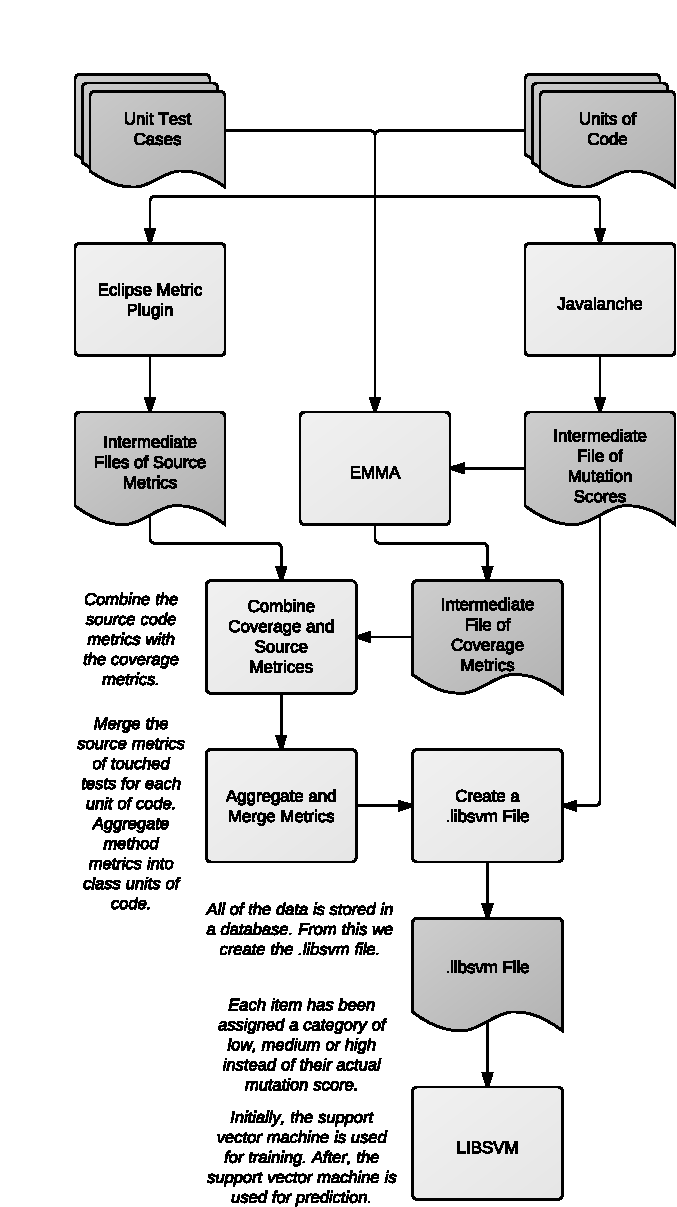
\includegraphics[width=7cm]{figures/process.pdf}
  \caption{Our SVM training process.}
  \label{fig:process}
\end{figure}


\section{Training}
\label{sec:training}
Our training process requires as input a set of units of code and for each code unit a corresponding set of unit test cases. Both the code units under test and test cases (i.e., JUnit tests) are Java source files.

The first step of our process is to collect the two types of data required to train the SVM:

\begin{itemize}
  \item \textbf{Category Data:} Javalanche is used to generate the mutants of all code units in the project under test and to perform the mutation testing by executing the required tests for each mutant. It should be noted that currently our Javalanche configuration does not exclude equivalent mutants from the analysis. For our research, we added a new analyzer component to Javalanche that outputs an intermediate text file of mutation scores of the covered units (methods and classes).

  \item \textbf{Feature Data:} The feature data is comprised of the source code and test suite metrics (see Table~\ref{tab:metrics} for feature sets referenced in the following text). By using the Eclipse Metric Plugin we collect source code metrics (sets \ding{172}~\&~\ding{174}) for both method- and class-level code units. We also collect the test suite metrics (set \ding{175}) of each unit's test cases using the Eclipse Metric Plugin. Test suite coverage metrics (set \ding{173}) are obtained using the EMMA tool.
\end{itemize}

Next, we create a .libsvm file containing the category and feature data from the database. Instead of predicting a specific mutation score percentage, we categorize all mutation scores as \textit{low, medium, high} which reduces the mutation score prediction to a three-group classification problem. The ranges of values in each category are determined based on the distribution of the mutation scores in our training data (further explained in Section~\ref{sec:results}). Finally, the .libsvm file is passed into LIBSVM to complete the training process.


\section{Prediction}
\label{sec:prediction}
Once we have trained the SVM, we can then use the SVM for prediction. We can predict the mutation score category of an unknown unit of code by first determining the source code and test suite metrics. The metrics (i.e., features) are passed into the SVM which will then assign a category of \textit{low, medium, high} for the mutation score.  Currently, our approach only predicts mutation scores within a project. That is, the training and prediction data both come from the same project repository.
